\chapter{Materials and Methods}\label{chap:methods}

\section{Galaxy Platform}\label{sec:galaxy}
Galaxy is a web-based scientific platform that has become a major player in many fields of life sciences and bioinformatics. Founded in 2007 it has provided an emerging amount of resources and tools to empower scientists and researchers to work with biomedical datasets. The platform is free to use and collaborative, making it one of the biggest of its kind. Resources on Galaxy cover genomics, metagenomics, transcriptomics, proteomics, drug discovery and non-biology fields like natural language processing and social sciences.

Galaxy's primary objective is to make analyses more accessible, reproducible, and easier to communicate among researchers. The platform's distinctive and success is attributed to four core elements: a very active community, a public server for analyses, an open-source software ecosystem, and the Galaxy ToolShed. The community adheres to the FAIR practices (Findable, Accessible, Interoperable and Reusable)~\cite{10.1093/nar/gkac247}.

The Galaxy community is thriving, with over 124,000 users who also contribute to subcommunities. The public server for analyses provides access to public datasets and workflows. The open-source software ecosystem ensures automated setup and deployment of all tools and services, making it simple for beginners and professionals to use. The Galaxy ToolShed is a server dedicated to hosting, sharing, and installing tools used on the platform. A Galaxy tool is the abstraction layer that makes external software usable from within Galaxy with a frontend, i.e. lets users use the program with all its parameters and inputs from within Galaxy. \\ 
Galaxy workflows are a key feature that allow the user to stack tools in a chain and to configure them so that the workflow user only has to upload his or her data for the input fields. The automation of tools in a chain is used for modular, longer analyses that are executed repeatedly. \\
Workflows that are available on and accepted by the Intergalactic Workflow Commission (IWC; \url{https://github.com/galaxyproject/iwc}) are conform with the community's best practise standards and tested on the latest Galaxy release. Dockstore and WorkflowHub automatically publish the IWC workflows and guarantee the availability in a Docker-based environment on Dockstore~\cite{o2017dockstore} and on the workflow collaboratory WorkflowHub~\cite{goble2021implementing}.

Important contributions of Galaxy, as stated by the Galaxy Community (2022), include Vertebrate Genome Project assembly workflows and collaborations on SARS-CoV-2 research. Another toolkit leveraged in Galaxy is Galaxy-ML, a set of tool that provides a suite for analyses based on machine learning. With growing publicity, more topics are covered by and moved to Galaxy. It has contributed to over 5,700 scientific publications and has many tutorials available for researchers to use. Training material and ready-to-use workflows facilitate professionals and beginners in the field to use Galaxy for their research purposes.

The platform is continuously enhanced, and it still attracts around 2,000 new users every month, indicating the quality and significance of the project. The team and infrastructure of Galaxy initially come from the Nekrutenko lab in the Center for Comparative Genomics and Bioinformatics at Penn State, the Taylor lab at Johns Hopkins University, and the Goecks Lab at Oregon Health \& Science University. All of these organisations have contributed significantly to the success of Galaxy. There are 138 public servers available worldwide as of 2023, while the most prominent general-purpose server instances are hosted by teams at University of Freiburg, Germany (for \href{https://usegalaxy.eu/}{UseGalaxy.eu}), Texas Advanced Computing Center (for \href{https://usegalaxy.org/}{UseGalaxy.org}) and Genomics Virtual Laboratory, formerly at the University of Queensland (for \href{https://usegalaxy.org.au/}{UseGalaxy.org.au}). These main public servers are synchronized in their tools and set of reference tools~\cite{10.1093/nar/gkac247}.


\section{Workflow Design}

\subsection{SARS-CoV-2 Pipeline as Baseline}
annotated variants are of interest \\
description of basic steps

\begin{figure}
	\centering
	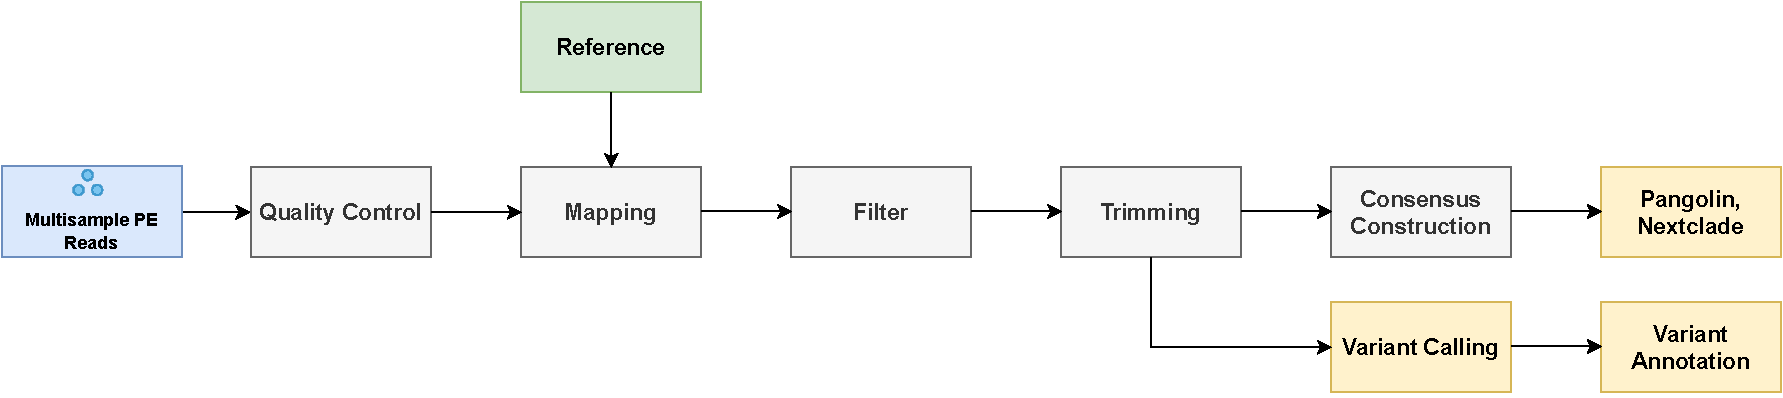
\includegraphics[width=0.97\textwidth]{media/3-pipelines-SARS-CoV-2.pdf}
	\caption{Simplified SARS-CoV-2 ARTIC PE reads iVar-based workflow.}
	\label{fig:3-pipelines-sars}
\end{figure}

well-established workflow, includes 'minimal' steps:
\begin{enumerate}
	\item Quality control
	\item Mapping
	\item Filtering
	\item Trimming
	\item Consensus Sequence Construction
\end{enumerate}

Plus Variant Calling and genome annotation; \\
Plus phylogenetic ranking ''to assign a SARS-CoV-2 genome sequence the most likely lineage based on a chosen nomenclature system'' (Pangolin)

\subsection{Requirements}

\begin{figure}
	\centering
	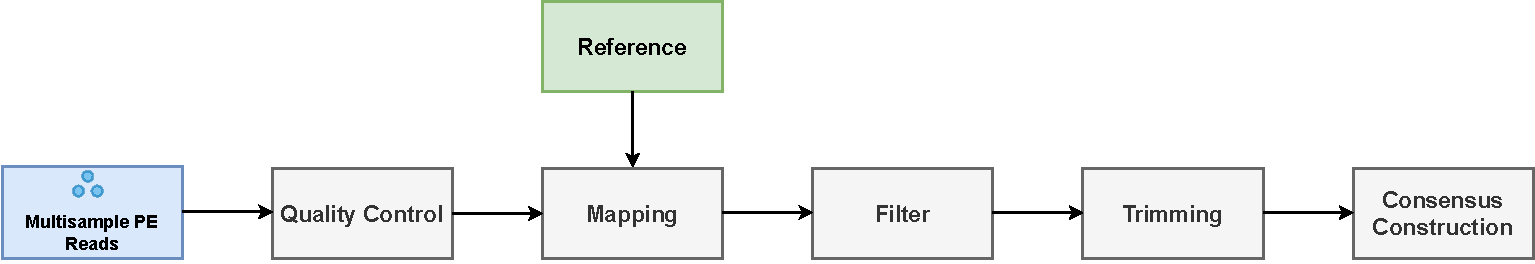
\includegraphics[width=0.97\textwidth]{media/3-pipelines-minimal.pdf}
	\caption{Simplified minimal ARTIC PE reads iVar-based workflow.}
	\label{fig:3-pipelines-minimal}
\end{figure}

which problems should the pipeline solve?

what is "ampliconic" sequence analysis, ARTIC Illumina-sequenced data

\subsubsection{Requirements for LSDV Workflow}
- repetitions in the start and end regions → need to split reads into 2 pools and mask references \\
- after splitting, merging alignments back

\subsubsection{Requirements for AIV Workflow}
- reference for each of the 8 segments has to be chosen \\
- align reference of each segment with consensus sequence for phylogenetic analysis \\
- snipit for visualisation of SNPs \\
- trimming would dismiss too many of the already short reads
\\ a tool to get closest reference

\section{Workflow Development}
"Reference-based genomic Surveillance" (INSaFLU)

\subsection{Pox Virus Illumina Amplicon Workflow}

Tiling amplicon approach for CaPV genome. Makes up 23 primer pairs for an amplicon size of 7.5 kb each instead of smaller sizes usually used in tiling amplicon protocols.

Workflow is composed of seven crucial steps:
- preparing reference sequence for mapping (masking halves)
- quality control
- mapping
- Filtering
- merging
- trimming
- consensus sequence construction

LSDV genome has its central coding region bounded by identical inverted terminal repeats,
containing 156 putative genes. the repeat of the ITRs would make any mapping in these regions ambiguous.
need to part the reads in two pools and do mapping in two parts: N-mask the  reference 

\begin{figure}
	\centering
	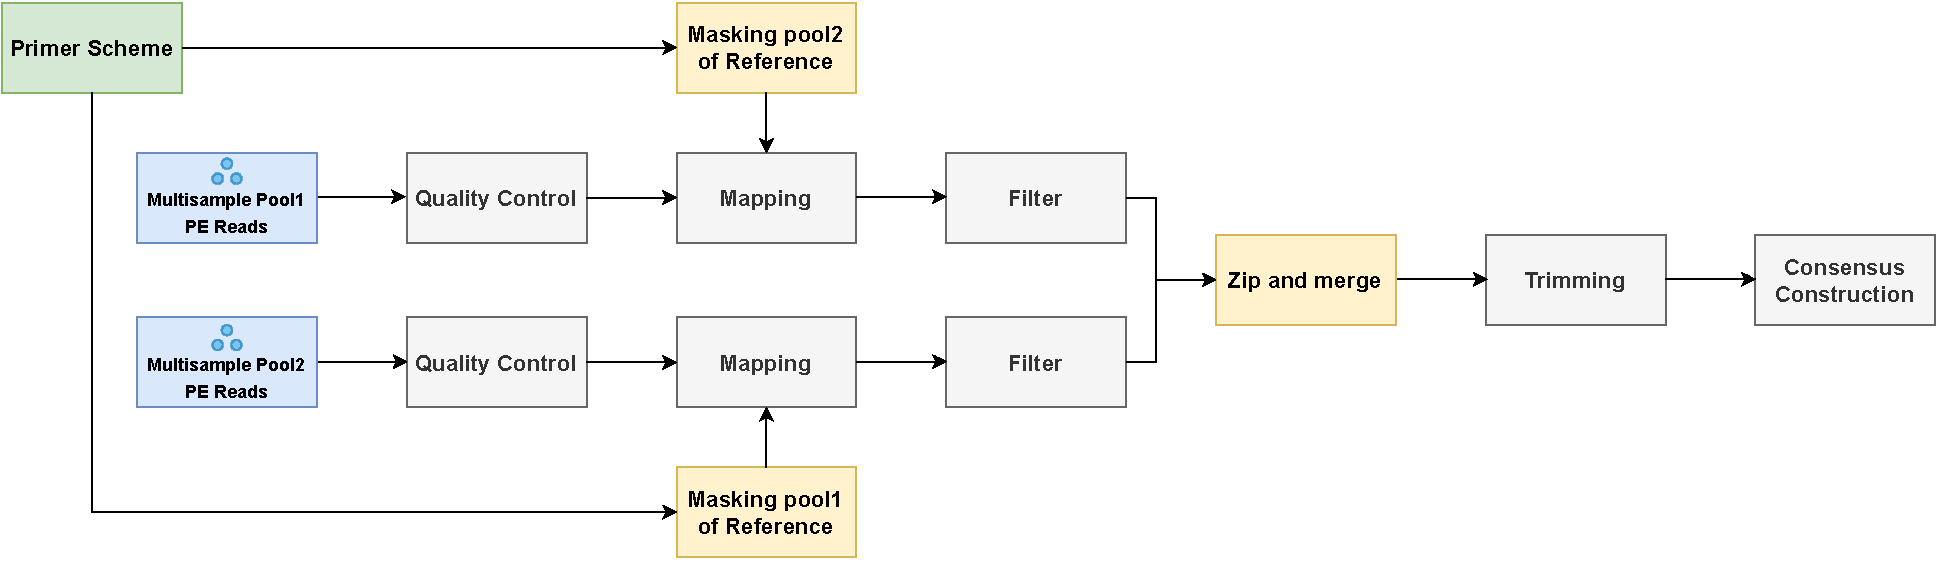
\includegraphics[width=0.97\textwidth]{media/3-pipelines-LSDV.pdf}
	\caption{Simplified LSDV ARTIC PE reads iVar-based workflow.}
	\label{fig:3-pipelines-lsdv}
\end{figure}

Efficiency: Assembly vs. Mapping!!; efficiency (hier nur kurz, ausführlicher in Diskussion). Wenn Ziel viele Samples/flächendeckende Überwachung ist, dann ist Assembly zu teuer. Im großen Stil soll das hier genutzt werden)

building index is expensive (BWT)

\subsection{AIV Illumina Amplicon Workflow}

explain VAPOR here

Kraken2 vs. VAPOR;
Efficiency: LoFreq vs. iVar consensus; both consensus identification methods using the same site-specific depth threshold

\begin{figure}
	\centering
	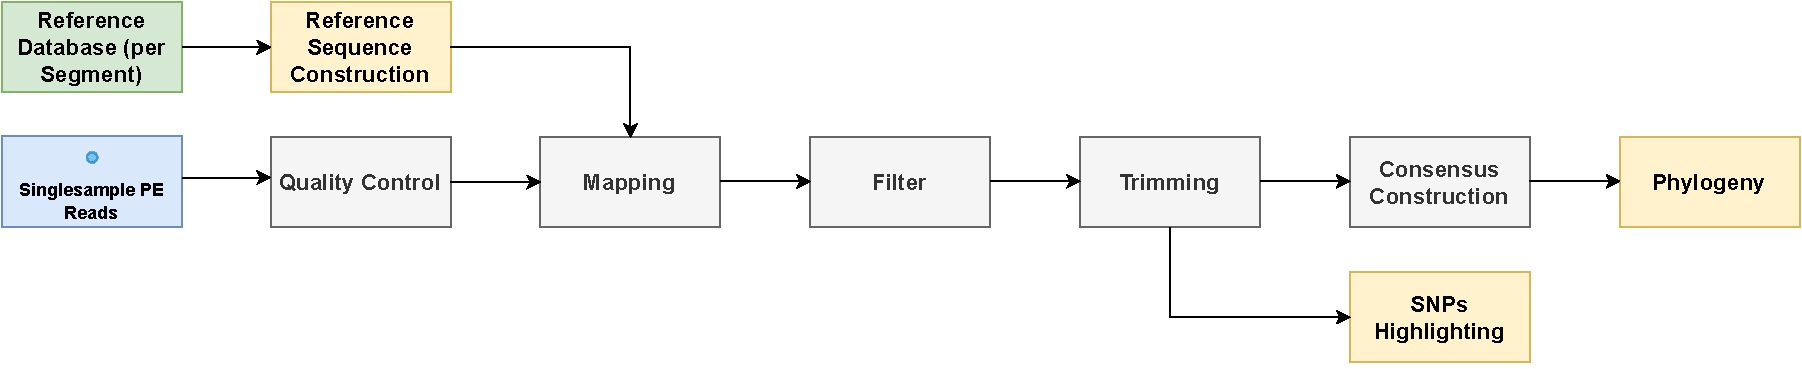
\includegraphics[width=0.97\textwidth]{media/3-pipelines-AIV.pdf}
	\caption{Simplified AIV ARTIC PE reads iVar-based workflow.}
	\label{fig:3-pipelines-aiv}
\end{figure}

\section{Workflow Evaluation}
\subsection{Evaluation of AIV Workflow Using Test Datasets}
 Sciensano s4+s8, Tunesian?

\subsection{Evaluation of Pox Virus Workflow Using LSDv Test Dataset}
 Sciensano by Elisabeth Mathijs
